\documentclass[11pt, a4paper, titlepage]{article}
\usepackage[left=2cm, right=2cm, top=2cm, bottom=2cm]{geometry}
\usepackage[style=authoryear,dashed=false,backend=bibtex]{biblatex}
\bibliography{MiniProject}
\usepackage{graphicx}
\usepackage{lineno}
\usepackage{csvsimple}
\usepackage{datatool}
\linespread{1.5}

\begin{document}

\begin{titlepage} % Suppresses headers and footers on the title page
	
	\centering % Centre everything on the title page
	
	\scshape % Use small caps for all text on the title page
	
	\vspace*{\baselineskip} % White space at the top of the page
	
	%------------------------------------------------
	
	%	Title
	
	%------------------------------------------------
	
	\rule{\textwidth}{1.6pt}\vspace*{-\baselineskip}\vspace*{2pt} % Thick horizontal rule
	
	\rule{\textwidth}{0.4pt} % Thin horizontal rule
	
	\vspace{0.75\baselineskip} % Whitespace above the title
	
	{\LARGE A comparison of a phenomenological model with Holling's mechanistic models for functional responses, focusing on consumer foraging movement\\} % Title
	
	\vspace{0.75\baselineskip} % Whitespace below the title
	
	\rule{\textwidth}{0.4pt}\vspace*{-\baselineskip}\vspace{3.2pt} % Thin horizontal rule
	
	\rule{\textwidth}{1.6pt} % Thick horizontal rule
	
	\vspace{2\baselineskip} % Whitespace after the title block
	
	%------------------------------------------------
	
	%	Subtitle
	
	%------------------------------------------------
	
	Computational Methods in Ecology and Evolution MRes
	\vspace{0.5\baselineskip}
	
	 MiniProject % Subtitle or further description
	
	\vspace*{3\baselineskip} % Whitespace under the subtitle
	
	%------------------------------------------------
	
	%	Editor(s)
	
	%------------------------------------------------
	
	\vspace{0.5\baselineskip} % Whitespace before the editors
	
	{\scshape\Large Lucy Goodyear\\
		Department of life Sceinces \\
		Imperial College London\\} % Editor list
	
	\textit{lucy.goodyear19@imperial.ac.uk}
	\date{}
	
	\vspace*{3\baselineskip} % Whitespace under the subtitle
	
	Word Count:
	
\end{titlepage}
	
\section*{Abstract}

\newpage

\linenumbers
\section{Introduction}
The term functional response refers to the relationship between a consumer's consumption rate and the density of its prey \parencite{Solomon1949}. 

The first mechanistic mathematical approach to functional responses was conducted by Holling in 1959 \parencite{Holling1959b}. Holling constructed an artifical functional response experiment and discovered that the funtional response was related to prey in terms of two constants, instantaneous rate of discovery and handling time. The instaneous rate of discovery is the likelihood of a predator finding an individual prey, equivalent to the volume or area searched per unit of time.
The handling time is any time not spent in actively searching for prey. There have been discussions on the different physical activites that handling time includes, such as digestion,time spent consuming prey, time spent hunting prey etc. \parencite{Jeschke2002, Holling1966}.

Holling desribed the three functional response...\parencite{Holling1959a} with the basic functional response becoming classed as a type II.

The Type III functional response was modeled using computer simulations and labeled as the generalised functional response by Holling 1965? \parencite{Holling1965} with Types I and II being limiting conditions. However, Type III was not described mathematically until 1977 by Real, who derived it using Holling's Type II functional response equation and first-order kinetic interations \parencite{Real1977}
 
The Generalised Functional Response equation is written below, where $c$ is the consumer response, $a$ is the instaneous rate of discovery, $x$ is the resource density, $h$ is the handling time and $q$ is a variable with as yet unknown biological meaning. It has been hyptohesised that q could be related to predator learning and is "the number of encounters...a predator must have with a prey item before becoming maximally efficient at utilizing the prey item as a resource" \parencite{Real1977}. In his paper, Real mathemaitcally derives the Type III (or generalised) functional response from looking at the kinetics \parencite{Real1977}.

\begin{equation}
c = \frac{ax_R^{q + 1}}{1 + hax_R^{q + 1}}
\end{equation}

It can been shown that the Type II functional response is a special case of the Generalised Functional Response by setting $q = 0$. In terms of Real's interpretation of $q$, the predator is "is always maximally efficient on the prey item"  \parencite{Real1977} in a Type II response.

\begin{equation}
c = \frac{ax_R}{1 + hax_R}
\end{equation}

 In Type I, the handling time is negligble, reducing the second term in the denominator to almost zero, leaving us with a linear relationship:

\begin{equation}
c = ax_R
\end{equation}

Type I responses are to be found in filter feeders, where the predation rate is directly  proportional to the prey density \parencite{Jeschke2004}. There is normally a hard cut off at very high prey densities. This because filter feeders are able to do activites simultaneous so can effectively spend all their time foraging.

The Holling model was then generalised in ... 
by .... to what is known as the generalised functional response model by including variable q. . 

This paper aims to look at the difference of fit between one such phenomological model (a polyomial) with the generalised functional response equation, a mechanistic model. The polynomial has no biological meaning so the comparison is effectly one of phenomological vs mechanistic models. 
Holling also discusses other attempts at modelling functional responses, remarking on the lack of biological context in most of the other options. \parencite{Holling1965}

By fitting the general functional response model to 308 datasets and comparing it to a polynomial fit, we can categorise the data, noticing the patterns that match the different data subsets. We can also compare functional response types by subsetting by limiting conditions of $h$ and $q$ respectively, gaining information on Type 1 and Type 2 Holling functional responses.

The second part of this paper will focus on comparing filter feeders and non-filter feeders. In pervious work, filter feeders have been shown to be more likely to show a Type 1 functional response. Jeschke et al showed that the Type 1 reponse was in fact exclusive to filter feeders \parencite{Jeschke2004}.  Functional responses that show a Type 1 respnse are characterised by 2 main confidtions: handling time must be negligible and satiation \parencite{Jeschke2002}. Many filter feeders have a negligible handing time because they are able to ctach prey at the same time as other activies so can effectlively spend all their time forgaing. Some filter feeders also adhere to the satiation condition but many don't, which is why the majority of all fucntional respnses, incuding filter feeders, do not show a type 1 response \parencite{Jeschke2004, Deville2013, Porter1983}. Our data set explores this in terms of Real's kinetic paper, looking at the responses when q is given no limit. \parencite{Real1977}

\section{Methods}

\subsection{Computing Tools}

Data was prepared for fitting using R. Rstudio makes it very easy to view data and i.... First the data was subsetted by the necessary columns and all records with NA trait value were discarded. This subset was run through a for loop to check that each ID had more than 5 records (the minimum number required for the fit with the most parameters (the cubic). Each ID was then plotted and saved to a single pdf in order to be able to give a quick review of the data. The data preparation script also generates the initial starting values for the general functional response fit, which are saved in the dataframe. The new dataframe, included subsetted data and initial starting values for a and h, is saved to csv for python load.

The starting value optimisation and fitting script is done using python. For the polynomial fit, there is an in-built python function, which also finds starting values for you. For the general functional response fit, a Gaussian sample of 100 was generated around the estimated starting values and each of these sample values was used to fit the model. The AIC, BIC and residual sums of sqaures (RSS) were calculated for each ID and the starting values for the model with the lowest AIC were chosen as the best fit. AIC was chosen over BIC because.....and when the number of estimated parameters is the same for each model (such as with GFR), choosing AIC is the equivalent of choosing RSS ...reference here. This loop is run for every ID.

Functions are saved in a separate python script and have been generalised to allow importation into future programmes. In python, the packages \textit{lmfit}, \textit{numpy} and \textit{pandas} were used. numpy contains the polynomial fitting function as well as the different mathematical values, such as pi. lmfit allows the use of parameters when fitting a model and pandas is a dataframe tool.

The best fit parameters and measured for all IDs are stored in a separate data frame and saved as a csv to be imported by the analsysi script, which has been done R due to the ease of data and graphical representation in R-studio. The analysis script plots each ID's datapoints, polynomial and generalised functional response fits. It compares RSS, AIC and BIC for each model within each ID. Based on the chosen best model for each ID, the IDs are then grouped and compared using the metadata.

\subsection{Statistics}

Three fit statistics were calculated to ensure each ID had a best fit model with two out of three agreements. AIC, BIC and RSS were calculated per each model for each ID. RSS was used as is rather than to calculate $R^{2}$ due to the new numerous pitfalls in calculating this statistic for non-linear regressions \parencite{kvalseth1985}. These were compared and the model with 2 or more out 3 agreements between the statistics was chosen as the best fit for that ID. AIC and BIXC were chosen because they are the best fitting statsitics \parencite{Johnson2004}.To obtain a measure of the significance of the results, both a G-test of goodness of fit and chi-square test of goodness of fit were performed.

\section{Results}

The findings of a comparison between the mechanistic model and the phenomenological models are shown in figure 1. It is clear that the mechanistic models are a much better fit. Only 0.7\% of the data was best fitted by phenomenological model, which accounts for 2 of 274 IDs. The superiority of the mechanistic models is highly signifctant ($p < 2.2\times10^{-16}$ for both chi-sqaure goodness of fit and G goodness of fit tests). 

Filter feeders and non-filter feeders are compared in figure 2. The ratio between the different best fits is similar to that of the whole dataset. It can also be seen that a small percentage non-filter feeder fucntional responses are best described by the Holling Type 1 functional response. Based on the paper of Jescke et al \parencite{Jeschke2004}, the expected proportions of Holling Type 1 response as best fit is 1 for filter feeders and 0 for non-filter feeders. These results are not insignifcant ($p < 2.2\times10^{-16}$ for both chi-sqaure goodness of fit and G goodness of fit tests). 

\begin{figure}[ht!]
	\centering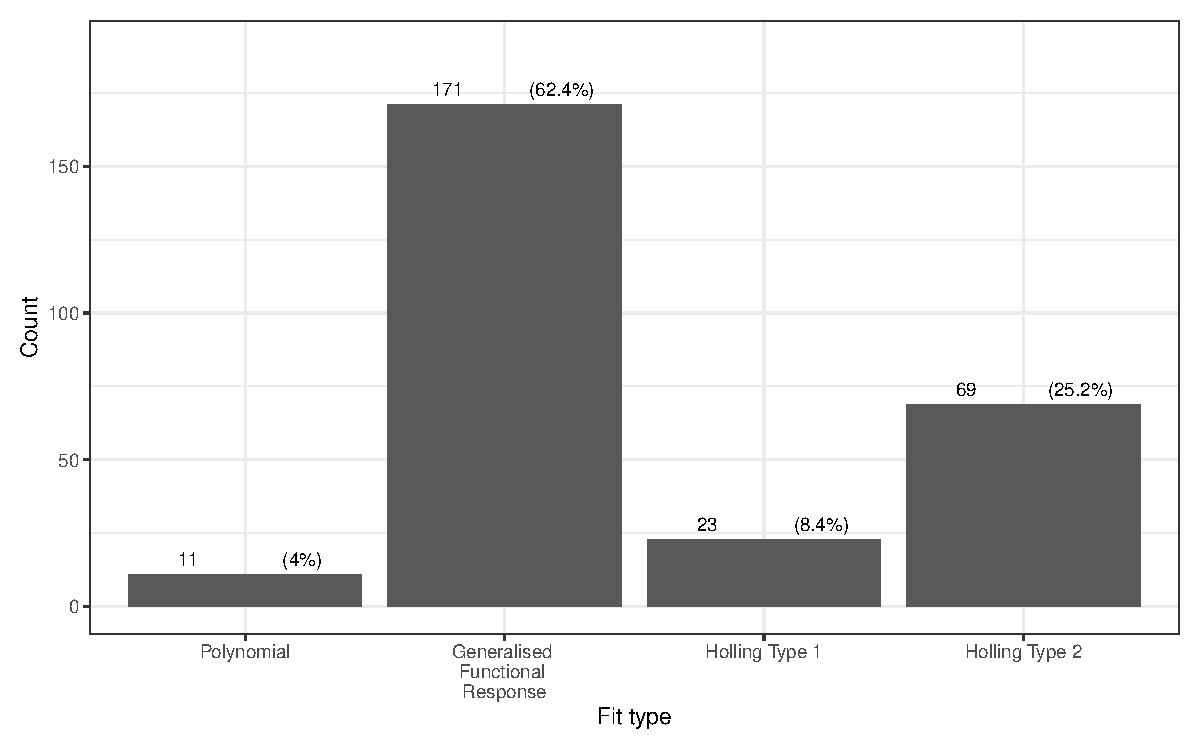
\includegraphics[width=1\textwidth]{../Results/Model_Comparison_Barchart.pdf}
	\caption{ID count by best fit type}
\end{figure}

\begin{table}[ht!]
\centering\csvreader[
respect all,
autotabular
]{../Results/sessilevsactivetable.csv}{}{\csvlinetotablerow}
\caption{Different fits by consumer foraging movement}
\end{table}

\begin{figure}[ht!]
	\centering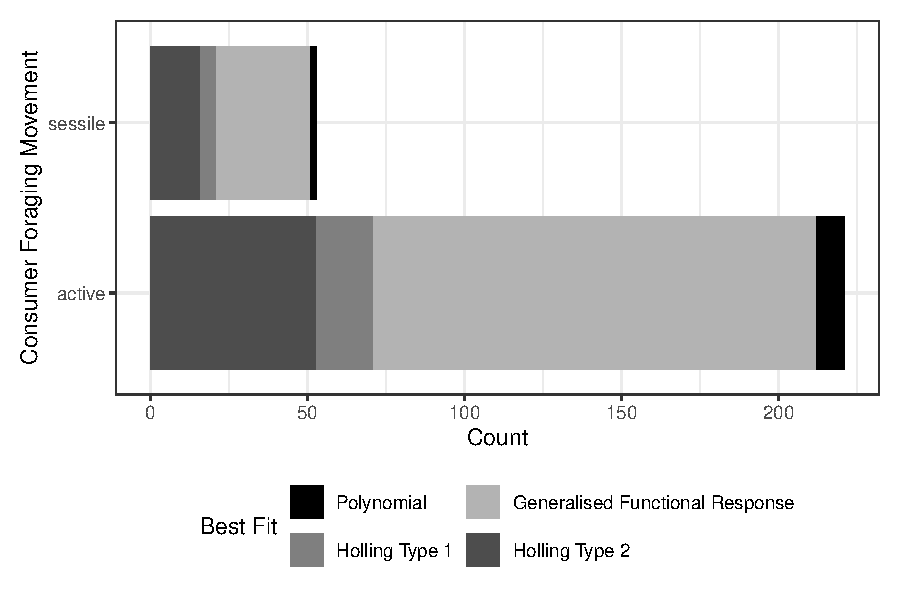
\includegraphics[width=0.9\textwidth]{../Results/ConForaging_Comparison_Barchart.pdf}
	\caption{ID count by best fit type}
\end{figure}

\section{Discussion}

As expected, the Holling mechanistic model much better explains fucntional response data than a polynomial. This is not to say that another mechanistic model would not describe the functional response with even more accuracy, however it does show the value of having models with biological basis.

The discrepancy between the expected number of non-filter feeders with a type 1 functional response could be explained in two ways:

1) Jeschke et al have a very broad definition of filter feeder, including that only filter feed at certain stages in their life cycle \parencite{Jeschke2004}. It could be that the authors of the data used a different defintion of filter feeder when classifying the consumer foraging type. However, this seems unlikely given that consumers have also been categorised by the lifestage in the dataset.

2) Both Holling Type 2 and 3 functional response are linear far from the limits. It is possible that not enough data has been collected at the limits to display a Type 2 or Type 3 functional response, which is why they have been interpretted as Type 1.

There is also work suggesting that functional response types change over spatial scales, which was not considered in the data analysed and could have impacted the results \parencite{Rincon2017}.

Further work has been done to refine the Holling models \parencite{Pawar2012, Seo2011, Aljetlawi2004} with modifications to account for both predator and prey size \parencite{Aljetlawi2004} and foraging dimensionality \parencite{Pawar2012}... and the work by Seo and DeAngelis in describing the Type I response shows a much more complicated dynamical system than once thought \parencite{Seo2011}

\newpage
\printbibliography

\end{document}